

\section{Business Intelligence Architectures}
\label{part:bi-architecture}
\begin{figure}[h]
    \centering
    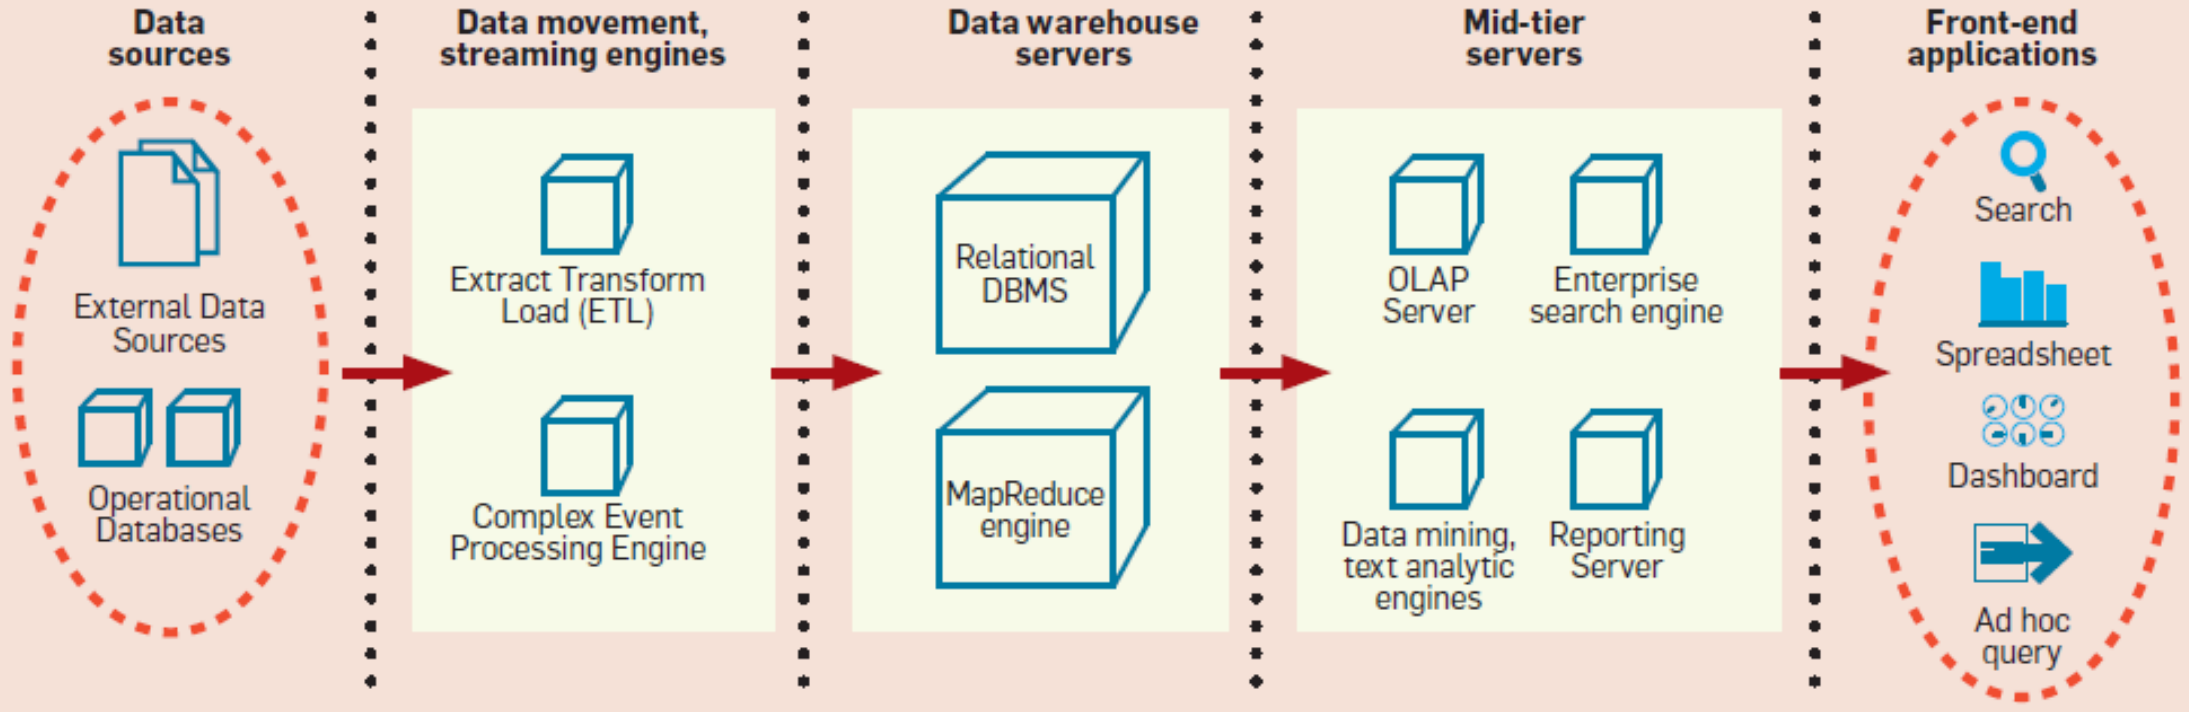
\includegraphics[width=\linewidth]{img/BI_ark.png}
        \caption{Architecture of a BI system.}
    \label{fig:bi-architecture}
\end{figure}

A Business Intelligence (BI) system turns raw operational data into information that supports decision-making. Its architecture is organized into five interconnected functional layers (Figure~\ref{fig:bi-architecture}):

\begin{enumerate}
    \item the \textbf{data sources} feed the system;
    \item the \textbf{ETL} layer extracts, transforms, and loads the data;
    \item the \textbf{data warehouse} stores it in integrated form;
    \item the \textbf{mid-tier servers} run advanced analysis;
    \item the \textbf{front-end applications} present the results.
\end{enumerate}

\subsection{Data Sources}
\label{sec:data-sources}

Data sources are the entry point of the BI architecture. An organization typically manages several operational sources spread across its departments, complemented by external feeds.

The data comes in heterogeneous formats: relational, multidimensional, documents, time series, spatial data, and real-time streams. This variety raises significant integration problems.

\subsection{Extract, Transform and Load}
\label{sec:etl-overview}

\begin{theorybox}
\textbf{ETL (Extract, Transform, Load)} is the process that extracts data from heterogeneous sources, transforms it to guarantee quality, consistency, and conformance to the target schema, and loads it into the data warehouse.
\end{theorybox}

The ETL process sits at the core of how the data warehouse is fed. Its three phases run in sequence: \textbf{extraction} retrieves the data from the sources; \textbf{transformation} cleans, normalizes, and enriches it; \textbf{loading} inserts it into the target structures.

Visual tools such as \textit{SQL Server Integration Services (SSIS)} simplify the design of complex ETL pipelines, letting a developer define transformation flows through drag-and-drop graphical interfaces.

\begin{figure}[h]
    \centering
    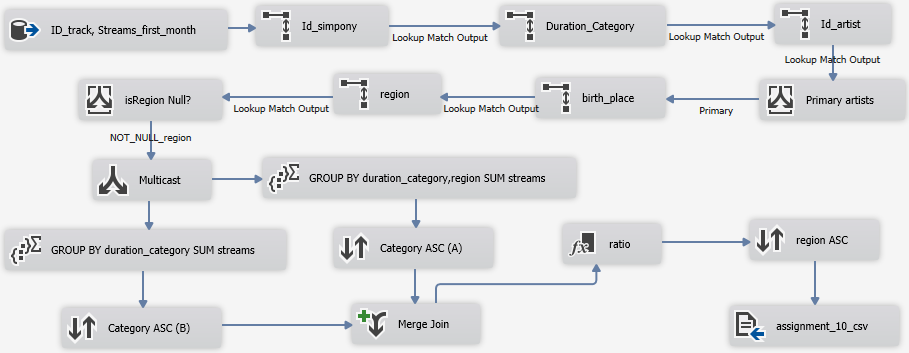
\includegraphics[width=0.85\linewidth]{img/assignment_10.png}
    \caption{An ETL pipeline.}
    \label{fig:etl-pipeline}
\end{figure}

Traditional ETL runs in \textbf{batch} mode: the data is processed within predefined time windows (nightly, weekly). This mode introduces latency but guarantees stability and control.

Modern scenarios often call for \textbf{incremental} or \textbf{real-time} processing. Incremental ETL processes only the data changed since the last run, cutting both time and resources.

\begin{theorybox}
\textbf{Complex Event Processing (CEP)} is a paradigm that analyzes continuous event streams in real time, identifies complex patterns through persistent queries, and produces immediate responses toward alerting systems, dashboards, or databases.
\end{theorybox}

\begin{figure}[h]
    \centering
    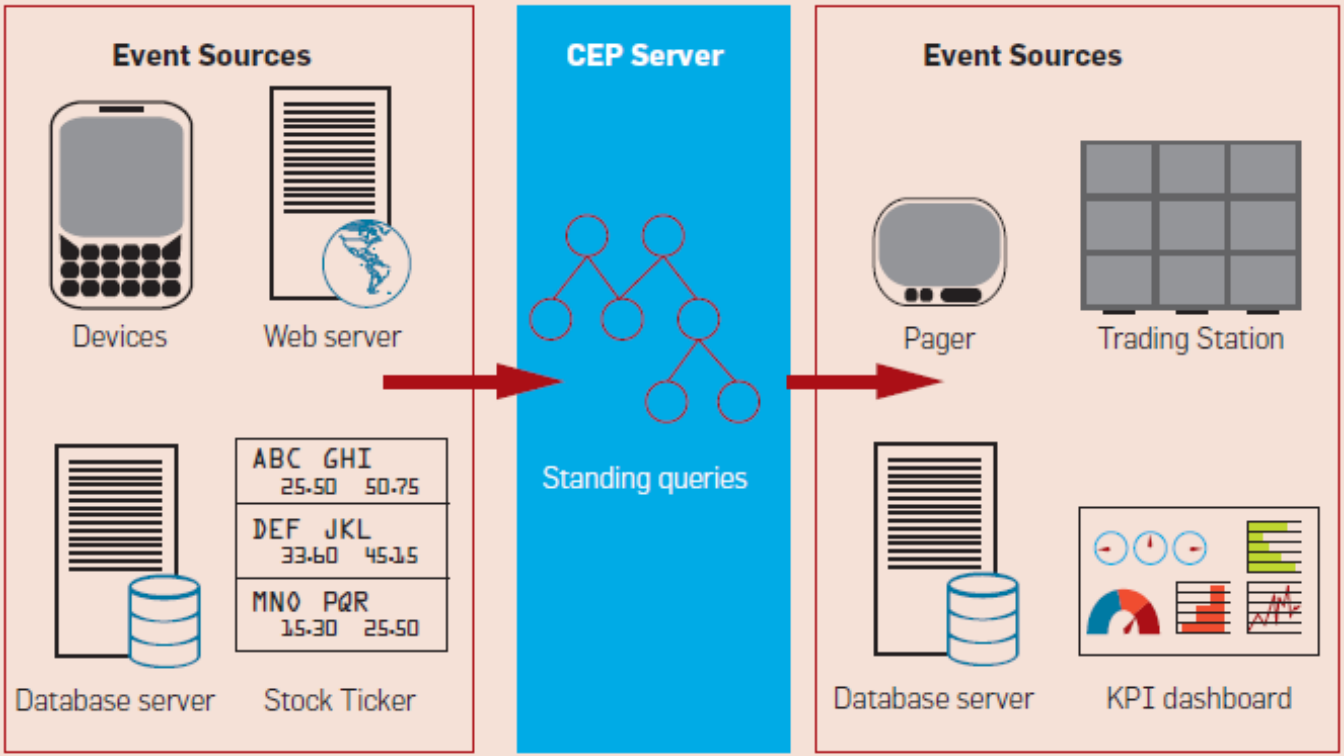
\includegraphics[width=0.9\linewidth]{img/CEP.png}
    \caption{CEP architecture: continuous streams from heterogeneous sources (IoT, web, databases) are processed by persistent queries to generate alerts and real-time updates.}
    \label{fig:cep-architecture}
\end{figure}

\subsection{Data Warehouse}
\label{sec:data-warehouse}

\begin{theorybox}
A \textbf{data warehouse} is a collection of data that supports decision-making processes, defined by four fundamental properties:
\begin{itemize}
    \item \textit{Subject-oriented}: the data is organized around the key concepts of the business (customers, products, sales) rather than around operational applications.
    \item \textit{Integrated}: data from heterogeneous sources is reconciled, made uniform in its encodings, and rendered consistent.
    \item \textit{Time-variant}: the data warehouse preserves the historical record of the data, enabling trend analysis and comparisons over time.
    \item \textit{Non-volatile}: loaded data is neither modified nor deleted; the warehouse operates read-only, with periodic insertions.
\end{itemize}
\end{theorybox}

The term \textit{data warehousing} denotes the entire process of designing, building, feeding, and using a data warehouse. Its typical structure follows a \textbf{dimensional schema} optimized for analytical queries.

\subsection{Data Warehouse Servers}
\label{sec:dw-servers}

The servers that host the data warehouse fall into two main categories: RDBMS optimized for analytical workloads, and distributed platforms for big data.

Relational databases built for data warehousing implement optimizations specific to analytical workloads, which are marked by complex queries over large volumes with few writes:

\begin{itemize}
    \item \textbf{Star-join optimization}: execution plans tuned for joins on star schemas, with efficient access to the fact table through the dimensional keys.
    \item \textbf{Bitmap index}: compressed indexes particularly effective on low-cardinality columns (e.g.\ gender, state, category), which are common in dimensions.
    \item \textbf{Partitioning}: horizontal partitioning of tables by date or another key, which limits scans to the relevant partitions only.
    \item \textbf{Materialized views}: pre-computed views that store the results of frequent aggregations, refreshed periodically.
    \item \textbf{Columnar storage}: organizing data by column instead of by row, which reduces I/O for queries that touch few attributes across many rows.
\end{itemize}

For volumes that exceed the capacity of individual servers, distributed platforms offer parallel processing on clusters of commodity hardware.

The \textbf{MapReduce} paradigm breaks processing into phases: \textit{Map} processes the input chunks in parallel, producing key-value pairs; \textit{Shuffle} redistributes the data, grouping it by key; \textit{Reduce} aggregates the values associated with each key. This model scales horizontally by adding nodes to the cluster.

\subsection{Mid-tier Servers}
\label{sec:mid-tier}

The mid-tier layer hosts services that turn the raw warehouse data into analytical information ready for consumption. It comprises OLAP servers, reporting engines, data mining engines, and enterprise search engines.

\begin{theorybox}
\textbf{OLAP (OnLine Analytical Processing)} provides a \textbf{multidimensional} view of the data, organized into structures called \textit{cubes} that allow interactive navigation along multiple dimensions of analysis.
\end{theorybox}

The user navigates the cube through intuitive operations: \textbf{drill-down} to increase detail, \textbf{roll-up} to aggregate, \textbf{slice} and \textbf{dice} to select subsets, and \textbf{pivot} to reorganize the display.
\begin{figure}[h]
    \centering
    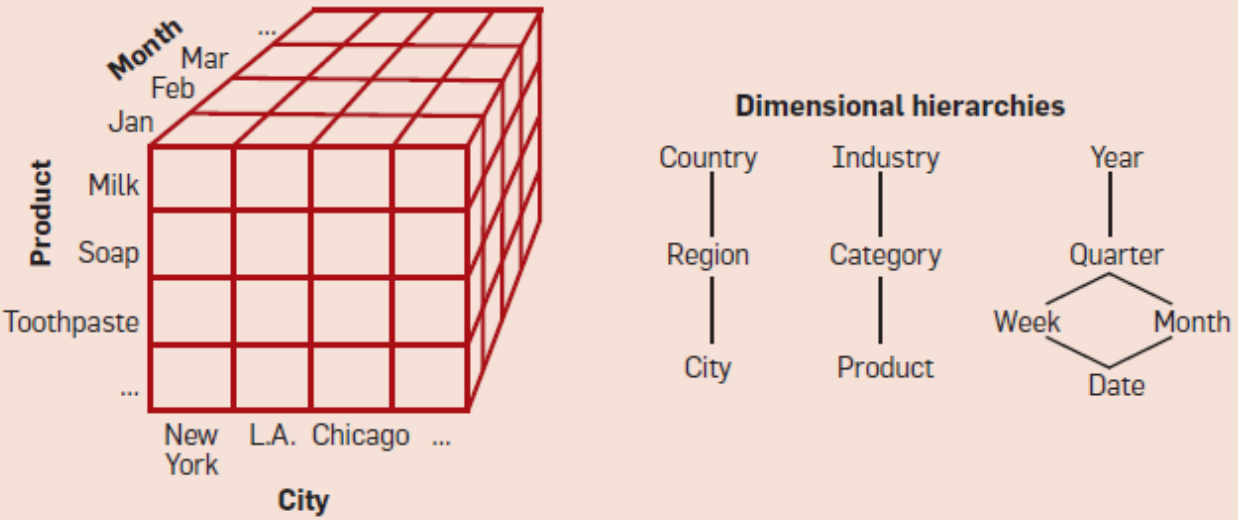
\includegraphics[width=0.9\linewidth]{img/cube_101.png}
    \caption{Representation of a multidimensional cube: measures (e.g.\ sales) can be analyzed along hierarchical dimensions (time, product, location).}
    \label{fig:olap-cube}
\end{figure}

\begin{theorybox}
\textbf{Reporting servers} manage the entire report lifecycle: parametric definition, scheduled execution, multi-format rendering (PDF, Excel, HTML, web), and automatic distribution via email or portals. The data is retrieved from the data warehouse or directly from the OLAP servers.
\end{theorybox}

\begin{theorybox}
\textbf{Data mining servers} extract patterns and predictive models from large data volumes. They support algorithms for classification, clustering, association, regression, and anomaly detection. Integration with the data warehouse allows mining techniques to be applied to consolidated historical data.
\end{theorybox}

\begin{theorybox}
\textbf{Enterprise search engines} index heterogeneous content (internal web pages, documents, email, structured data), enabling unified keyword search. Full-text indexing complements structured SQL/MDX queries.
\end{theorybox}

\subsection{Front-end Applications}
\label{sec:frontend}

Front-end applications form the interface between the BI system and its end users, offering access modes that differ by user profile and skill.

\begin{itemize}
    \item \textbf{Spreadsheets and pivot tables}: interactive navigation of multidimensional data in a familiar environment (Excel, Google Sheets). Pivot tables let the user place dimensions on rows and columns, apply filters, and expand or collapse hierarchies.
    \item \textbf{Dashboards and portals}: concise visualizations with KPIs, charts, and indicators that update automatically. Enterprise portals centralize access to reports and analytics.
    \item \textbf{Ad-hoc query tools}: interfaces for advanced users who build custom queries without resorting to SQL.
    \item \textbf{Vertical applications}: packaged solutions for specific domains, such as CRM analytics, supply chain optimization, financial reporting, and sentiment analysis.
    \item \textbf{Data storytelling}: tools that combine visualizations, annotations, and narrative to communicate insights in a form decision makers can grasp.
\end{itemize}
